\chapter{Modelle zur Gesten- und Spracherkennung}
\label{chap:Modelle}
% Einf\"uhrende Worte
Es existieren diverese Verfahren zur Gesten- und Spracherkennung. Die bekanntesten Vertreter sind \glspl{NeuroNetz}, \gls{DTW} und \gls{HMM}.
\newline
Im Folgenden werden kurz die diversen Eigenschaften und Algorithmen hinter den verschiedenen Verfahren er\"ortert, um eine fundierte Entscheidung \"uber die Auswahl eines dieser Modelle f\"ur diese Arbeit und das zu erarbeitende Programm zu treffen.

\section{Dynamic Time Warping}
\gls{DTW} ist ein Algorithmus zur Messung von \"Ahnlichkeiten zwischen einer Eingabesequenz und einem gegebenen Muster, die sich im zeitlichen Ablauf oder der Geschwindigkeit unterscheiden. Dabei w\"urden zum Beispiel die Gemeinsamkeiten im Laufmuster erkannt werden, selbst wenn eine Person in einem Video langsam l\"auft und diese Person in einer weiteren Aufnahme schneller laufen w\"urde, oder gar eine Beschleunigung oder Verlangsamung w\"ahrend des Zeitraumes der Beobachtung stattfindet.
\newline
Formalisiert versteht man unter \acrshort{DTW} eine vorlagenbasierte Erkennungstechnik auf Grundlage von \glslink{DP}{dynamischer Programmierung}~\cite[S.~963]{bib:hmmlee}.
Trotz der Erfolge bei Aufgaben mit kleinem Vokabular, braucht \acrshort{DTW} eine gro\ss e Anzahl an Vorlagen f\"ur ein gr\"osseres Umfeld an Variation. Weiterhin kann es keine undefinierten Muster verarbeiten.
\newline
Takahashi et al.~\cite{bib:takahashi} haben einen \textit{Erkundungsalgorithmus} vorgeschlagen, um Gesten des K\"orpers und der Arme zu erkennen. Lee beschreibt die Funktionalit\"at wie folgt: Ein Eingabemuster wird von einer Bildeingabesequenz zu jeder Zeit $t$ generiert. Dabei wird der Zeitpunkt $t$ als m\"oglicher Endpunkt der Geste betrachtet und das Eingabemuster mit allen vordefinierten Mustern verglichen. \gls{DP} wird dabei genutzt, um die Entfernung zwischen zwei Mustern zu berechnen, ungeachtet der zeitlichen Differenz.
\newline
Der Nachteil dieses Ansatzes ist die geringe Robustheit gegen\"uber Variationen der Form und Gestalt.

\section{K\"unstliche neueronale Netze}
Ein weiterer Ansatz ist die Nutzung von \glslink{KNN}{k\"unstlichen neuronalen Netzen}. Beale und Edwards~\cite{bib:beale} nutzten diese trainierbaren Erkennungssysteme zur Erkennung von Handgesten. Eine weitere Arbeit von Beale und Finlay~\cite{bib:finlay} nutzt diese Technik, denn sobald gro\ss e Datenmengen verf\"ugbar werden, um so mehr Relevanz erh\"alt der Einsatz von \glslink{KNN}{k\"unstlichen neuronalen Netzen}.\footnote{Vergleiche Lee und Kim~\cite{bib:hmmlee}.}
\newline
Ein Problem der neuronalen Netze im Kontext der Gestenerkennung ist jedoch die Modellierung von Mustern von \textit{Nichtgesten}. Trotz der Effektivit\"at bei der Erkennung von statischen Mustern, sind \gls{KNN}{k\"unstliche neuronale Netze} nach Vaananen und Boehm~\cite{bib:vaananen} nicht f\"ur dynamische Muster (Gesten) geeignet.

\section{Hidden Markov Model}
Das \gls{HMM} ist ein stochastisches Modell, in dem ein System durch eine Markov-Kette mit unbeobachteten Zust\"anden modelliert wird. Die Theorie dazu wurde von Baum~\cite{bib:hmmbaum}, 1966 ver\"offentlicht.
\newline
Es wird dazu angewendet, um Zeitreihen mit zeitlicher und r\"aumlicher Variabilit\"at zu analysieren. Dabei kann es auch mit undefinierten Mustern umgehen. Ein \gls{HMM} besteht dabei aus verschiedenen Komponenten.
\newline
Der versteckte (englisch \textit{hidden}) Prozess ist eine Markov-Kette und besteht aus Zust\"anden und \"Ubergangswahrscheinlichkeiten.
Das Modell ist wie folgt definiert:

\subsubsection{Definition}
Ein \gls{HMM} $\lambda = (S, A, O, B, \pi)$ ist gegeben durch
\begin{itemize}
  \item $S = {S_1,\ldots,S_n}$ -- Menge aller Zust\"ande,
  \item $A = {a_{ij}}$ -- \"Ubergangsmatrix zwischen den Zust\"anden, wobei $a_{ij}$ die Wahrscheinlichkeit angibt, dass Zustand $S_i$ in Zustand $S_j$ gewechselt wird,
  \item $O = {O_1,\ldots,O_m}$ -- Menge der m\"oglichen Beobachtungen (\textit{Emissionen}),
  \item $B = {b_{ij}}$ -- Beobachtungsmatrix, wobei $b_{ij}$ die Wahrscheinlichkeit angibt, im Zustand $S_i$ die Beobachtung $O_j \in O$
  \item $\pi$ -- Anfangswahrscheinlichkeitsverteilung mit $\pi (i)$ Wahrscheinlichkeit, dass $S_i$ der Startzustand ist.
\end{itemize}

\section{Auswahl des Modells f\"ur die Arbeit}
Rabiner et al.~\cite[S.~257f]{bib:hmmrabiner}, sowie Lee und Kim~\cite[S.~961]{bib:hmmlee} sprechen von den guten Erfolgen des \gls{HMM} als stochastisches Werkzeug zur Modellierung von Gesten. Die Autoren stimmen dieser Auffassung zu. Daher wird f\"ur diese Arbeit eine Implementierung mittels \acrshort{HMM} erarbeitet.

\section{Diskrete Markov-Prozesse}
\label{subsec:MarkovKette}
Eine Markov-Kette ist ein \gls{StochProz}. Dabei unterscheidet man zwischen Markov-Ketten in diskreter und in stetiger Zeit. Weiter spricht man von Markov-Ketten, sofern ein diskreter Zustandsraum vorhanden ist, von \textit{Markov-Prozessen} im Allgemeinen wenn ein stetiger Zustandsraum vorliegt.
\newline
Bei einem \acrshort{HMM} werden ausschlie\ss lich diskrete Markov-Ketten verwendet, die wie folgt definiert sind.

\subsubsection{Definition}
Gegeben sei ein System, das zu jeder gegebenen Zeit $t$ beschrieben werden kann, als sich in einer Menge von $N$ verschiedenen Zust\"anden
$S_1, S_2, \ldots, S_N$ befindend. Abbildung \ref{fig:MarkovKette} zeigt eine solche Markov-Kette mit f\"unf Zust\"anden $S_1$ bis $S_5$.
\begin{figure}[htb]
\centering
\includegraphics[width=5cm]{img/markov/markov_chain.png}
\caption[Markov-Kette mit f\"unf Zust\"anden]{Markov-Kette mit f\"unf Zust\"anden \protect{($S_1$ bis $S_5$)} mit Verbindungen (Quelle: \protect{\cite{bib:hmmrabiner}})}
\label{fig:MarkovKette}
\end{figure}
In regelm\"a\ss igen diskreten Zeitabst\"anden nimmt das System eine Zustands\"anderung vor, gem\"a\ss~einer Wahrscheinlichkeitsmenge, die mit dem Zustand verkn\"upft ist. Die Zeitinstanzen, die mit den Zustands\"anderungen verkn\"upft sind, werden durch $t = 1, 2, \cdots$ gekennzeichnet und der aktuelle Zustand zum Zeitpunkt $t$ als $q_t$. F\"ur den Fall, einer diskreten Markov-Kette erster Ordnung ist diese Charakterisierung ausreichend, da
\begin{equation}
\label{E:PropMarkov}
P[q_t = S_j | q_{t-1} = S_i, q_{t-2} = S_k, \cdots]= P[q_t = S_j | q_{t-1} = S_i].
\end{equation}
Weiterhin werden ausschlie\ss lich die Prozesse betrachtet, in denen die rechte Seite der Gleichung~\ref{E:PropMarkov} zeitunabh\"angig ist, was somit zur Menge der \"Ubergangswahrscheinlichkeiten $a_{ij}$ der Form
\begin{equation}
\label{E:PropTrans}
a_{ij} = P[q_t = S_j | q_{t-1} = S_i], 1 \leq i, j \leq N
\end{equation}
f\"uhrt, wobei die Zustands\"ubergangskoeffizienten folgende Eigenschaften erf\"ullen:
\begin{subequations}
\begin{align}
\label{E:MarkovProperties}
a_{ij} \geq 0 \\
\sum_{j = 1}^{N} a_{ij} = 1
\end{align}
\end{subequations}
Ein solcher \gls{StochProz} stellt aber noch kein \gls{HMM} dar.
\newline
Um ein besseres Verst\"andnis f\"ur diese Prozesse und deren Eigenschaften zu erlangen, wird im folgenden anhand eines Beispiels aus einer Anleitung von Lawrence Rabiner~\cite{bib:hmmrabiner} n\"aher auf das Thema eingegangen.
\newline
Man betrachte ein einfaches Markov Modell, dass mittels drei Stati das Wetter beschreibt. Diese drei Zust\"ande sind folgende:
\begin{itemize}
\item[Status 1:] Regnerisch
\item[Status 2:] Bew\"olkt
\item[Status 3:] Sonnig
\end{itemize}
Es wird gefordert, dass das Wetter am Tag $t$ durch einen der drei oberen Zust\"ande beschrieben wird. Weiter wird die Matrix $A$ der Wahrscheinlichkeiten der Zustands\"uberg\"ange wie folgt definiert:
\[
\label{E:MarkovProbMatrix}
\mathbf{A} = {a_{ij}} = 
\begin{pmatrix}
0,4 & 0,3 & 0,3 \\
0,2 & 0,6 & 0,2 \\
0,1 & 0,1 & 0,8 \\
\end{pmatrix}
\]
Das Wetter am ersten Tag $( t = 1)$ sei als sonnig (Status 3) gegeben. Stellt man nun die Frage, nach der Wahrscheinlichkeit f\"ur eine Folge von Wetterzust\"anden, oder anders formuliert, f\"ur einen Wetterverlauf der n\"achsten sieben Tage, wie \enquote{sonnig, sonnig, regnerisch, regnerisch, sonnig, bew\"olkt, sonnig,\ldots}, so kann man hierzu formal eine Sequenz aus mehreren Zust\"anen betrachten. Hierzu sei die Beobachtungssequenz $O$ definiert als $O = {S_3, S_3, S_1, S_1, S_3, S_2, S_3}\,$, was mit $t = 1, 2, \cdots, 8$ \"ubereinstimmt. Die Wahrscheinlichkeit kann ausgedr\"uckt werden als,
\begin{align}
P(O|Modell) &= P[S_3, S_3, S_3, S_1, S_1, S_3, S_2, S_3| Modell] \notag \\
 &= P[S_3] \cdot P[S_3|S_3] \cdot P[S_3|S_3] \cdot P[S_1|S_3] \cdot P[S_1|S_1] \cdot P[S_3|S_1] \cdot P[S_2|S_3] \cdot P[S_3|S_2] \notag \\
 &= \pi _3 \cdot a_{33} \cdot a_{33} \cdot a_{33} \cdot a_{31} \cdot a_{11} \cdot a_{13} \cdot a_{32} \cdot a_{23}\notag \\
 &= 1 \cdot (0,8) (0,8) (0,1) (0,4) (0,3) (0,1) (0,2)\notag\\ 
 &= 1,536 \times 10^{-4}, \notag
\end{align}
wobei
\begin{align} \label{E:PropMarkovWetterPi}
\pi _i = P[q_1 = S_i]\, , & & 1 \leq i \leq N
\end{align}
die Wahrscheinlichkeit f\"ur den initialen Status darstellt.
\newline
Auch die Frage nach der Wahrscheinlichkeit wie lange das Modell in einem gegebenen und bekannten Status genau $d$ Tage verbleibt, kann mittels \gls{HMM} beantwortet werden. Dabei kann die Wahrscheinlichkeit durch die Beobachtungssequenz
\begin{equation}
O = {\underset{1}{S_i}, \underset{2}{S_i}, \underset{3}{S_i}, \cdots, \underset{d}{S_i}\, , \underset{d+1}{S_j} \ne S_i} \notag
\end{equation}
ermittelt werden:
\begin{equation}
\label{E:PropMarkovD}
P(O | Modell,\, q_1 = S_i) = (a_{ii})^{d-1}(1 - a_{ii}) = p_i(d)
\end{equation}
Die Gr\"o\ss e $p_i(d)$ ist die (diskrete) Wahrscheinlichkeitsdichtefunktion der Dauer $d$ im Status $i$. Diese ist charakteristisch f\"ur die Dauer eines Status in einer Markov-Kette. Basierend auf $p_i(d)$ kann man die erwartete Zahl der Betrachtungen (Dauer) in einem Status berechnen, unter der Voraussetzung, dass in diesem Status gestartet wird, mit
\begin{subequations}\label{E:MarkovDuration}
    \begin{alignat}{2}
      \overline{d_i} &= \sum_{d= 1}^{\infty} dp_i(d)\label{E:MarkovDuration1}\\
      &= \sum_{d = 1}^{\infty} d(a_{ii})^{d - 1} (1 - a_{ii}) = \frac{1}{1 - a_{ii}} \, . \label{E:MarkovDuration2}
    \end{alignat}
  \end{subequations}
Daraus ergeben sich die Anzahl aufeinander folgender Sonnentage, gem\"a\ss \, dem Modell $\frac{1}{0,2} = 5$,  die Anzahl aufeinanderfolgender bew\"olkter Tage entsprechend mit $2,5$ und die Anzahl aufeinanderfolgender Regentage mit $1,67$.

\subsection{Erweiterung auf Hidden Markov Model}
\label{subsec:HMM}
% in einzelne Abschnitte aufteilen
Um Markov Prozesse auf Probleme anwenden zu k\"onnen, in denen sich die Beobachtungen nicht auf Zustand beziehen, muss das bisher dargestellte Konzept erweitert werden. Dazu wird der Fall hinzugef\"ugt, dass eine Beobachtung durch eine Wahrscheinlichkeitsfunktion des Zustandes ausgedr\"uckt wird. Nach Rabiner~\cite{bib:hmmrabiner} besteht das resultierende Modell aus einem doppelt eingebetteten stochastischen Prozess mit einem darunter liegenden, nicht beobachtbaren(versteckten, daher \textit{hidden}), \glslink{StochProz}{stochastischen Prozess} und wird als \gls{HMM} bezeichnet.
\newline
Ein \acrshort{HMM} ist wie folgt charakterisiert:
\begin{enumerate}
\item Sei $N$ die Anzahl aller Zust\"ande im Modell, dann sind die verschiedenen Zust\"ande definiert als $S = {S_1, S_2, \cdots, S_N}$ und der Zustand zum Zeitpunkt $t$ ist definiert als $q_t$.
\item Sei $M$ die Anzahl aller verschiedenen Beobachtungssymbole pro Zustand, dann sind die individuellen Symbole definiert als $V = {v_1, v_2, \cdots, v_M}$.
\item Sei $A = {a_{ij}}$ die \"Ubergangsmatrix, wobei
\begin{align}
a_{ij} = P[q_{t+1} = S_j \mid q_t = S_i] \, , & & 1 \leq i, j \leq N \, .
\end{align}
F\"ur den speziellen Fall, dass jeder beliebige Zustand jeden beliebigen anderen Zustand in einem Schritt erreichen kann, ist $a_{ij} > 0$ f\"ur alle $i, j$. F\"ur alle weiteren Typen eines \acrshort{HMM} ist $a_{ij} = 0$ f\"ur mindestens ein $(i, j)$ Paar.
\item Sei $B = {b_j(k)}$ die Beobachtungsmatrix im Zustand $j$, wobei
\begin{align}
b_j(k) = P[v_k \,\mbox{zum Zeitpunkt} \, t \mid q_t = S_j]\, , & & 1 \leq j \leq N \, \, \, \,  \notag \\
& & \, \, 1 \leq k \leq M \, .
\end{align}
\item Sei $\pi = {\pi_i}$ die Anfangswahrscheinlichkeitsverteilung, wobei
\begin{align}
\pi_i = P [q_1 = S_i] \, , & & 1 \leq i \leq N \, .
\end{align}
\end{enumerate}
Sind entsprechende Werte f\"ur $N, M, A, B$ und $\pi$ gesetzt, so kann das \acrshort{HMM} als Generator verwendet werden, um eine Beobachtungssequenz 
\begin{equation}
O = O_1 \, O_2 \, \cdots \, O_T
\end{equation}
wie folgt zu erhalten:
\begin{enumerate}
\item W\"ahle einen Startzustand $q_1 = S_i$ entsprechend der Anfangswahrscheinlichkeitsverteilung $\pi$ .
\item Setze $t = 1$ .
\item W\"ahle $O_t = v_k$ entsprechend der Beobachtungsmatrix f\"ur den Zustand $S_i$, das hei\ss t, $b_i(k)$.
\item Gehe in in einen neuen Zustand $q_{t+1} = S_j$ entsprechend der Beobachtungsmatrix f\"ur den Zustand $S_i$ \"uber, das hei\ss t, $a_{ij}$.
\item Setze $t = t+ 1$; kehre zu Schritt 3 zur\"uck, falls $t < T$; beende andernfalls die Prozedur.
\end{enumerate}
Nach Rabiner~\cite[S. 5]{bib:hmmrabiner} kann diese Prozedur sowohl dazu verwendet werden, Beobachtungen zu generieren und als Modell, wie eine gegebene Beobachtungssequenz von einem entsprechendem \acrshort{HMM} erstellt wurde.
\newline
Eine vollst\"andige Spezifikation eines \acrshort{HMM} ben\"otigt die Beschreibung zweier Modellparameter ($N$ und $M$), die Spezifikation von Beobachtungssymbolen und die Beschreibung der drei Wahrscheinlichkeitsgr\"o\ss en $A, B$ und $\pi$.
Meist wird hierf\"ur die kompakte Notation
\begin{equation}
\lambda = (A, B, \pi)
\end{equation}
verwendet, um die Vollst\"andigkeit aller Parameter des Modells anzuzeigen.

\subsection[Die drei grundlegenden Probleme eines Hidden Markov Model]{Die drei grundlegenden Probleme eines Hidden
\label{subsec:HMMProbleme}
 Markov Model \protect{\footnote{Die Ausf\"uhrungen basieren auf den Vortr\"agen von Jack Ferguson von IDA an den Bell Laboratories}}}
Verwendet man die oben ausgef\"uhrte Form eines \acrshort{HMM}, die in Abschnitt~\ref{subsec:HMM} beschrieben ist, so ergeben sich drei grundlegende Probleme, die vor einem Einsatz von \gls{HMM} in einer Anwendung gel\"ost werden m\"ussen. Diese lauten wie folgt:
\begin{enumerate}
\item[Problem 1:] Sind die Beobachtungsmenge $O = O_1 \, O_2 \, \cdots \, O_T$ und ein Modell $\lambda = (A, B, \pi)$ gegeben, wie kann dann die Wahrscheinlichkeit der Beobachtungsmenge, $P( O \mid \lambda)$, effizient berechnet werden, sofern das Modell gegeben ist?
\item[Problem 2:] Sind die Beobachtungsmenge $O = O_1 \, O_2 \, \cdots \, O_T$ und ein Modell $\lambda$ gegeben, wie w\
"ahlt man dann eine entsprechende Zustandsfolge $Q = q_1 \, q_2 \, \cdots \, q_T$ die f\"ur das gew\"unschte Resultat optimal ist?
\item[Problem 3:] Wie sind die Parameter des Modells $\lambda =(A, B, \pi)$ anzupassen, um $P ( O \mid \lambda)$ zu maximieren?
\end{enumerate}
Im folgenden sind Verfahren und Techniken aufgef\"uhrt, wie die soeben genannten Probleme gel\"ost werden k\"onnen.

\subsection{Das Vorw\"arts--R\"uckw\"artsverfahren}
Das Vorw\"arts--R\"uckw\"artsverfahren~\cite{bib:baum}~\cite{bib:sell}~\cite{bib:hmmrabiner} erm\"oglicht eine L\"osung des ersten Problems aus Abschnitt~\ref{subsec:HMMProbleme} \footnote{Zur L\"osung des Problems 1 wird lediglich der Verw\"artsteil des Verfahrens ben\"otigt, der R\"uckw\"artsteil wird im Problem 3 ben\"otigt, aber dennoch hier behandelt}:
Betrachtet man die Vorw\"artsvariable $\alpha_t(i)$, definiert als
\begin{equation}
\alpha_t(i) = P (O_1 \, O_2 \, \cdots \, O_t\,,\, q_t = S_i \mid \lambda)
\end{equation}
d.h., die Wahrscheinlichkeit der partiellen Menge der Beobachtungen, $O_1 \, O_2 \, \cdots \, O_t$, (bis Zeitpunkt $t$) und Zustand $S_i$ zum Zeitpunkt $t$, bei gegebenem Modell $\lambda$. Induktiv ist dies wie folgt l\"osbar:
\begin{itemize}
\item[1) Induktionsanfang:]
\begin{align}
\alpha_1(i) = \pi_i b_i (O_1) \, , & & 1 \leq i \leq N \, .
\end{align}
\item[2) Induktionsschritt:]
\begin{align}
\label{E:forwardIS}
\alpha_{t+1}(j) = \left[\sum_{i = 1}^{N} \alpha_t(i) a_{ij} \right] b_j (O_{t+1}) \, , & & 1 \leq t \leq T - 1 \, \, \, \,\notag \\
 & & 1 \leq j \leq N \, .
\end{align}
\item[3) Induktionsschluss:]
\begin{equation}
P( O \mid \lambda) = \sum_{i = 1}^{N} \alpha_T(i) \, .
\end{equation}
\end{itemize}
Der Induktionsanfang initialisiert die Vorw\"artswahrscheinlichkeit als die kombinierte Wahrscheinlichkeit des Zustands $S_i$ und der Anfangsbeobachtung $O_1$. Der Induktionsschritt ist Kern des Vorw\"artsalgorithmus und ist dargestellt in Abbildung~\ref{fig:ForwardVariable}(a).
\begin{figure}[htb]
\centering
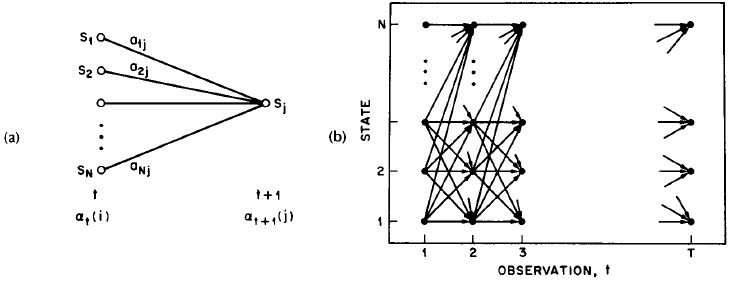
\includegraphics[width=\textwidth]{img/markov/forward_variable.png}
\caption[(a) Illustration der Oerpationsfolge zur Berechnung der Vorw\"artsvariable.(b) Implementierung der Berechung von  $\alpha_t(i)$ im Netz der Beobachtungen $t$ und Zust\"ande $i$.]{(a) Illustration der Oerpationsfolge zur Berechnung der Vorw\"artsvariable $\alpha_{t+1}(j)$.~(b) Implementierung der Berechung von $\alpha_t(i)$ im Netz der Beobachtungen $t$ und Zust\"ande $i$. (Quelle: \protect{\cite{bib:hmmrabiner}})}
\label{fig:ForwardVariable}
\end{figure}
Die Abbildung zeigt wie der Zustand $S_j$ zum Zeitpunkt $t + 1$ von den $N$ m\"oglichen Zust\"anden $S_i \,,\, i \leq i \leq N$ vom Zeitpunkt $t$ aus erreicht werden kann. Das Produkt $\alpha_t(i) a_{ij}$ stellt die Wahrscheinlichkeit des gemeinsamen Ereignisses dar, dass $O_1 \, O_2 \, \cdots \, O_t$ beobachtet wurden und Zustand $S_j$ von $S_i$ aus erreicht wurde. Das Aufsummieren des Produkts ergibt die Wahrscheinlichkeit f\"ur $S_j$ mit allen fr\"uheren partiellen Beobachtungen. Die Berechnung von~\ref{E:forwardIS} wird f\"ur alle Zust\"ande $j$ durchgef\"uhrt. Abschlie\ss end ergibt der Induktionsschluss die gew\"unschte L\"osung von $P( O \mid \lambda)$ als die Summe der terminalen Vorw\"artsvariablen $\alpha_T(i)$. Das ist der Fall, da laut Definition,
\begin{equation}
\alpha_T(i) = P (O_1 \, O_2 \, \cdots \, O_T \, , \, q_T = S_i \mid \lambda)
\end{equation}
und somit $P (O \mid \lambda)$ lediglich die Summe der $\alpha_T(i)$'s ist.
\newline
Die Vorw\"artswahrscheinlichkeitsberechnung basiert auf der Gitterstruktur, die in Abbildung~\ref{fig:ForwardVariable}(b) dargestellt ist. Der Schl\"ussel liegt darin, da nur $N$ Zust\"ande (Knoten zu jedem Zeitintervall im Gitter) existieren, fallen alle m\"oglichen Zustandsfolgen, wieder in diese $N$ Knoten, ungeachtet der L\"ange der Beobachtungsfolge.
\newline
In \"ahnlicher Weise kann eine R\"uckw\"artsvariable $\beta_t(i)$ definert werden, als
\begin{equation}
\beta_t(i) = P ( O_{t+1} \, O_{t+2} \, \cdots \, O_T \mid q_t = S_i \, , \, \lambda)
\end{equation}
d.h., die Wahrscheinlichkeit der partiellen Beobachtungsfolgen von $t + 1$ bis zum Ende, gegeben dem Zustand $S_i$ zum Zeitpunkt $t$ und dem Modell $\lambda$.
\newline
Ebenfalls induktiv wird $\beta_t(i)$ wie folgt gel\"ost:
\begin{itemize}
\item[Induktionsanfang:]
\begin{align}
 \beta_T(i) = 1 \, , & & 1 \leq i \leq N \, .
\end{align}
\item[Induktionsschritt:]
\begin{align}
\beta_t(i) = \sum_{j = 1}^{N} a_{ij} b_{j} (O_{t + 1}) \beta_{t + 1} (j) \, , & & t = T - 1, T - 2, \cdots , 1 \, \, \, \,  \notag \\
& & 1 \leq i \leq N \, .
\end{align}
\end{itemize}
Der Induktionsschritt definiert $ \beta_T(i)$ willk\"urlich als $1$ f\"ur alle $i$. Der Induktionsschritt, dargestellt in Abbildung~\ref{fig:BackwardVariable}, zeigt, dass man um im Zustand $S_i$ zum Zeitpunkt $t$ gewesen zu sein, man alle m\"oglichen Zust\"ande $S_j$ zum Zeitpunkt $t + 1$ ber\"ucksichtigen muss.
\newline
Die Berechnung von $\beta_t(i)$ kann ebenfalls in einer Gitterstruktur, \"ahnlich der in Abbildung~\ref{fig:ForwardVariable}(b) durchgef\"uhrt werden.
\begin{figure}[htb]
\centering
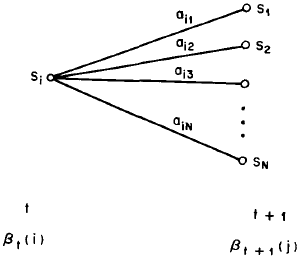
\includegraphics[width=0.35\textwidth]{img/markov/backward_variable.png}
\caption[Illustration der Oerpationsfolge zur Berechnung der R\"uckw\"artsvariable.]{Illustration der Oerpationsfolge zur Berechnung der R\"uckw\"artsvariable $\beta_{t}(i)$. (Quelle: \protect{\cite{bib:hmmrabiner}})}
\label{fig:BackwardVariable}
\end{figure}

\subsection{Anmerkungen zu Problem 2}
Anders als f\"ur Problem 1, kann f\"ur Problem 2 aus Abschnitt~\ref{subsec:HMMProbleme} keine exakte L\"osung angegeben werden. Dennoch gibt es mehrere Ans\"atze das Problem 2 hinsichtlich einzelner Kriterien zu l\"osen. Zum Einen kann nach Rabiner~\cite{bib:hmmrabiner} die \enquote{optimale} Zustandsfolge verbunden mit der gegebenen Beobachtungsfolge gefunden werden. Die Schwierigkeit liegt bei der Definition der optimalen Zustandsfolge, das hei\ss t, es gibt verschiedene m\"ogliche Optimierungskriterien. Ein m\"ogliches Optimierungskriterium ist, die Zust\"ande $q_t$ zu w\"ahlen, die \textit{individuell} am wahrscheinlichsten sind. Um dies umzusetzen, wird die Variable
\begin{equation}
\label{E:DefGamma}
\gamma_t(i) = P (q_t = S_i \mid O \, , \, \lambda)
\end{equation}
definiert, das hei\ss t, die Wahrscheinlichkeit zum Zeitpunkt $t$ im Zustand $S_i$ zu sein, bei gegebener Beobachtungsfolge O und Modell $\lambda$. Gleichung~\ref{E:DefGamma} kann mittels Vorw\"arts--R\"uckw\"arts Variablen ausgedr\"uckt werden, d. h.,
\begin{equation}
\label{E:FracGamma}
\gamma_t(i) = \frac{\alpha_t(i) \beta_t(i)}{P (O  \mid \lambda)} = \frac{\alpha_t(i) \beta_t(i)}{\sum_{i = 1}^{N} \alpha_t(i) \beta_t(i)}
\end{equation}
wobei $\alpha_t(i)$ f\"ur die partielle Beobachtungsfolge $O_1 \, O_2 \, \cdots \, O_t$  und  und Zustand $S_i$ zum Zeitpunkt $t$ steht, w\"ahrend $\beta_t(i)$ f\"ur die restliche Beobachtungsfolge $O_{t +1} \, O_{t + 2} \, \cdots \, O_T$ steht, sofern Zustand $S_i$ bei $t$ gegeben ist. Der Normierungsfaktor $P (O  \mid \lambda) = \sum_{i = 1}^{N} \alpha_t(i) \beta_t(i)$ macht $\gamma_t(i)$ zu einer Wahrscheinlichkeitsgr\"o\ss e, so dass 
\begin{equation}
\sum_{i = 1}^{N} \gamma_t(i) = 1 \, .
\end{equation}
Benutzt man $ \gamma_t(i)$, so kann man f\"ur den individuell wahrscheinlichsten Zustand $q_t$ zum Zeitpunkt $t$ l\"osen, als
\begin{align}
\label{E:argmaxGamma}
q_t =  \underset{1 \leq i \leq N}{\argmax} [\gamma_t(i)] \, & & 1 \leq t \leq T \, .
\end{align}
Trotz der Tatsache, dass Gleichung~\ref{E:argmaxGamma} die erwartete Anzahl an korrekten Zust\"anden maximiert, k\"onnen Probleme in den resultierenden Zustandsfolgen auftreten, da lediglich der wahrscheinlichste Zustand in jedem Moment bestimmt wird, ungeachtet der Wahrscheinlichkeit des Auftretens von Zustandsfolgen.
\newline
Daher wird meist ein anderes Optimierungskriterium verwendet, das Auffinden der \textit{einzelnen} besten Zustandesfolge, d. h., die Maximierung von $P (Q \mid O \, , \lambda)$. Die Technik, diese beste Zustandsfolge zu finden, basiert auf \glslink{DP}{dynamischer Programmierung} und ist der sogenannte Viterbi Algorithmus~\cite{bib:viterbi}~\cite{bib:forney}.
\newline
Dieser spielt f\"ur diese Arbeit aber keine Rolle und wird daher nicht weiter betrachtet. F\"ur weitere Informationen wird auf die Literatur verwiesen.

\subsection{Baum-Welch-Algorithmus}
Das dritte und bei weitem schwierigste Problem eines \gls{HMM}, ist die Bestimmung einer Methode zur Anpassung der Modellparameter $(A, B, \pi)$, um die Wahrscheinlichkeit der Beobachtungssequenz eines gegebenen Modells zu maximieren.
\newline
Es ist laut Rabiner~\cite[S.~264]{bib:hmmrabiner} kein analytisches Verfahren zur L\"osung des Problems bekannt. Es ist jedoch m\"oglich, so Rabiner weiter, ein $\lambda = (A, B, \pi)$ so zu w\"ahlen, dass $P (O \mid \lambda)$ lokal maximiert wird. Das bekannteste Verfahren hierzu ist der sogenannte Bauch-Welch-Algorithmus~\cite{bib:baumFellow}~\cite{bib:baumWelch}.
\newline
Rabiner~\cite[S.~264ff]{bib:hmmrabiner} stellt hierzu eine detaillierte Beschreibung des Algorithmus bereit.

\subsection{Typen des Hidden Markov Model}
Bislang wurde lediglich der Spezialfall eines sogenannten \glslink{Ergo}{\textit{ergodischen}} oder vollst\"andig verbundenen \acrshort{HMM}s betrachtet, wobei jeder Zustand des Modells von jedem anderen Zustand des Modells aus (in einem Schritt) erreicht werden. (Streng mathematisch gesprochen: in einer finiten Anzahl von Schritten). Wie in Abbildung~\ref{fig:HMMTypes}(a) zu sehen, hat dieses $N = 4$ Zustandsmodell, die Eigenschaft, dass jeder $a_{ij}$ Koeffizient positiv ist. Aus dem Beispiel in Abbildung~\ref{fig:HMMTypes}(a) erhalten wir
\begin{equation}
\mathbf{A} = 
\begin{pmatrix}
a_{11} & a_{12} & a_{13} & a_{14} \\
a_{21} & a_{22} & a_{23} & a_{24} \\
a_{31} & a_{32} & a_{33} & a_{34} \\
a_{41} & a_{42} & a_{43} & a_{44} \\
\end{pmatrix} \, .
\end{equation}

\begin{figure}[htb]
\centering
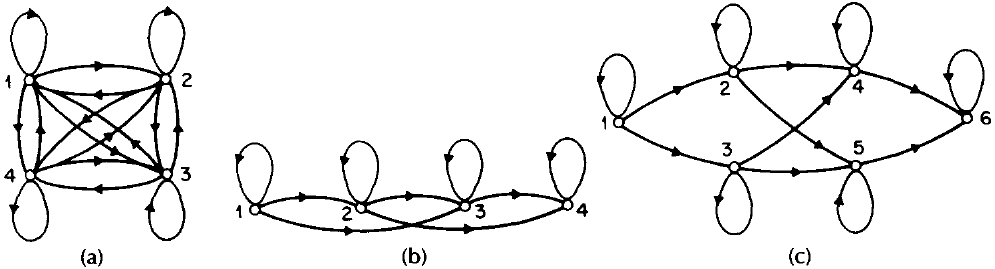
\includegraphics[width=\textwidth]{img/markov/markov_types_h.png}
\caption[Darstellung dreier verschiedener Typen eines HMMs. (a) 4-Zustand ergodisches Modell. (b) 4-Zustand links-rechts Modell. (c) 6-Zustand Parallelpfad links-rechts Modell]{Darstellung dreier verschiedener Typen eines HMMs. (a) 4-Zustand ergodisches Modell. (b) 4-Zustand links-rechts Modell. (c) 6-Zustand Parallelpfad links-rechts Modell. (Quelle: \protect{\cite{bib:hmmrabiner}})}
\label{fig:HMMTypes}
\end{figure}

Andere Typen von \acrshort{HMM}s bieten bessere Beobachtungseigenschaften des Signals und stellen sich f\"ur einige Anwendungen daher als besser modelliert heraus, als das \glslink{Ergo}{ergodische} Modell. Eines dieser Modelle ist das aus  Abbildung~\ref{fig:HMMTypes}(b). Dieses Modell ist ein sogenanntes links-rechts Modell oder Bakis Model~\cite{bib:jelinek}~\cite{bib:bakis}, da die dahinter liegende Zustandsfolge, die mit dem Modell verbunden ist, die Eigenschaft hat, dass sofern die Zeit zunimmt, der Zustandsindex zunimmt (oder gleich bleibt), d. h., die Zust\"ande verlaufen von links nach rechts. Die fundamentale Eigenschaft aller links-rechts HMMs ist, dass die Zustands\"ubergangskoeffizienten die Eigenschaft
\begin{align}
a_{ij} = 0 \, , & & j \leq i
\end{align}
besitzen, d. h., keine \"Uberg\"ange zu Zust\"ande, deren Indizes kleiner als der gegenw\"artige sind, sind zugelassen. Weiter haben die Anfangswertwahrscheinlichkeiten folgende Eigenschaft
\[
\pi_i = 
\begin{cases}
	0, & i \ne 1 \\
	1, & i = 1
\end{cases}
\]
nachdem die Zustandsfolge im Zustand $1$ starten (und im Zustand $N$ enden) muss. Bei links-rechts Modellen werden oft weitere Bedingungen an die Zustands\"ubergangskoeffizienten gekn\"upft, um sicher zustellen, dass gro\ss e \"Anderungen in den Zustandsindizes nicht auftreten; daher wird folgende Bedingung h\"aufing verwendet:
\begin{align}
a_{ij} = 0 \, , & & j > i + \varDelta \, .
\end{align}
Insbesondere f\"ur das Beispiel aus Abbildung~\ref{fig:HMMTypes}(b), ist $\varDelta$ gleich $2$, das hei\ss t, keine Spr\"unge \"uber mehr als zwei Zust\"ande sind zul\"assig. Die \"Ubergangsmatrix f\"ur dieses Beispiel sieht demnach wie folgt aus:
\begin{equation}
\mathbf{A} = 
\begin{pmatrix}
a_{11} & a_{12} & a_{13} &0 \\
0 & a_{22} & a_{23} & a_{24} \\
0 & 0 & a_{33} & a_{34} \\
0 & 0 & 0 & a_{44} \\
\end{pmatrix}
\end{equation}
Dabei sollte klar sein, dass f\"ur den letzten Zustand in einem links-rechts Modell, die Zustands\"ubergangskoeffizienten definiert sind, als
\begin{subequations}
\begin{align}
\label{E:TransitionProperties}
a_{NN} &= 0  \\
a_{Ni} &= 0 \, , & & i < N \, . 
\end{align}
\end{subequations}
Daneben existieren nat\"urlich noch zahlreiche weitere Variationen und Kombinationen von Modelltypen. Als Beispiel hierf\"ur zeigt Abbildung~\ref{fig:HMMTypes}(c) eine doppelt \"uberkreuzte Verbindung zweier paralleler links-rechts HMMs.